\documentclass{article}
\usepackage[T1]{fontenc}
\usepackage{lmodern}
\usepackage{graphicx}
\usepackage{amsmath,amssymb}
\usepackage[a4paper,margin=2cm]{geometry}
\usepackage[absolute,overlay]{textpos}
\setlength{\TPHorizModule}{1mm}
\setlength{\TPVertModule}{1mm}
\usepackage[indonesian]{babel}
\usepackage{hyperref}
\setlength{\emergencystretch}{2em}
% unit: Halaman 15

\begin{document}

% === Halaman 15 (llm) ===

\vspace{172.26mm}

\vspace{10mm}
\begin{itemize}
    \item Dua huruf yang paling sering muncul di dalam cipherteks: huruf P dan Z.
    \item Dua huruf yang paling sering muncul di dalam B. Inggris: huruf E dan T.
    \item Kemungkinan besar,
    \begin{itemize}
        \item P adalah pemetaan dari e
        \item Z adalah pemetaan dari t
    \end{itemize}
    \item Tetapi kita belum dapat memastikannya sebab masih diperlukan cara \textit{trial and error} dan pengetahuan tentang Bahasa Inggris.
    \item Tetapi ini adalah langkah awal yang bagus.
\end{itemize}

% deskripsi: Tabel frekuensi kemunculan 1-gram yang menampilkan Rank, 1-gram, Absolut, dan Relatif.
% bbox normalisasi: [0.0280, 0.1800, 0.4300, 0.7600]
\begin{textblock*}{84.42mm}(5.88mm,53.46mm)
\noindent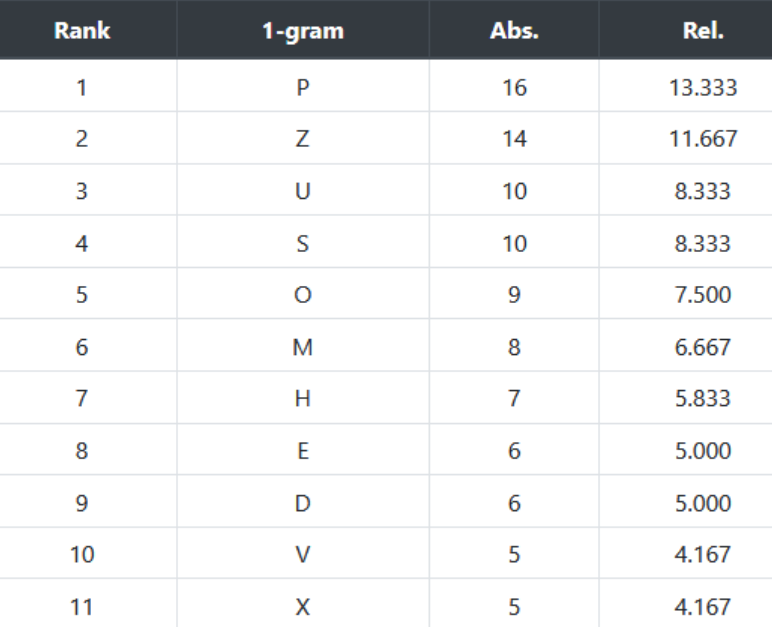
\includegraphics[width=84.42mm,height=172.26mm]{../../images/llm/page_015_img_01.png}%
\end{textblock*}

\end{document}
